\chapter{Nicht ganzzahlige Flüsse}

Wie in Kapitel \ref{main_algo} erwähnt, impliziert eine nicht ganzzahlige Lösung für ein Multi-Fluss-Problem auf einem gerichteten Graphen mit $n\geq 2$ Paaren von Quellen und Senken, im Allgemeinen nicht die Existenz einer ganzzahligen Lösung. Die Ergebnisse aus Kapitel \ref{the_program}, lassen jedoch die Möglichkeit offen, dass das man in unserem Fall die folgende Vermutung beweisen kann. Wir wollen uns deswegen in diesem Kapitel mit der von Aerts und Felsner offen gelassenen Frage beschäftigen, ob die Erkennung von Graphen mit einer SLTR in $\mathcal{P}$ liegt.

\begin{conjecture}\label{int_conj}
Sei $\tilde{\varphi}=(\tilde{\varphi_1},\tilde{\varphi_2})$ ein nicht ganzzahliger zulässiger Fluss auf $\mathcal{N}_G$, dann existiert auch eine ganzzahlige Lösung $\varphi$ und wir können in linearer Zeit ein Gutes-FAA aus $\tilde{\varphi_2}$ extrahieren, ohne eine ganzzahlige Lösung zu berechnen.
\end{conjecture}

\begin{remark}
Wenn wir nicht darauf bestehen, dass unsere Lösung ganzzahlig ist, dann lässt sich eine Lösung nach TODO durch lineare Programmierung in polynomineller Zeit finden und das Entscheidungsproblem, ob ein Graph eine SLTR hat läge so in $\mathcal{P}$.
\end{remark}

Um die Argumentation einfacher zu gestalten, werden wir unser 2-Fluss Problem manchmal als 3-Fluss Problem, mit einer Lösung $\varphi=(\varphi_s,\varphi_e,\varphi_z)$, betrachten. Wir erstellen also $\mathcal{N}_G^*$, wie zuvor $\mathcal{N}_G$, nur mit drei Quellen und Senken und weisen Schnyder-, Zuweisungs- und Ecken-Fluss eigene Typen zu. Man kann leicht sehen, dass Theorem \ref{theo_algo} in angepasster Form hier ebenfalls gilt und ein zulässiger  Fluss $(\varphi_s,\varphi_e,\varphi_z)$ auf $\mathcal{N}_G^*$ genau dann existiert, wenn auch ein zulässiger Fluss $(\varphi_1,\varphi_2)$ auf $\mathcal{N}_G$ existiert. Die Hinrichtung ist klar. Nehmen wir an $(\varphi_1,\varphi_2)$ ist eine ganzzahlige Lösung. Nach Beobachtung A2 gilt, dass die äusseren Kanten eines Winkel-Dreiecks entweder von einem Ecken- oder einem Zuweisungs-Pfad genutzt werden. Diese Kanten sind, zusammen mit den Kanten von Quelle 2 zu den Winkeldreiecken, die einzigen in $\mathcal{N}_G$ die von beiden Flüssen genutzt werden. Wir können also $\varphi_2$ in $|\varphi_2|$ ganzzahlige Pfade aufteilen und jeden Pfad entweder $\varphi_e$ oder $\varphi_z$ zuweisen, je nachdem ob er über die Dummy-Senke führt, oder nicht. Insbesondere folgt mit der gleichen Argumentation:  

\begin{itemize}
\item [O1] Jede beliebige Kombination von $\varphi_s,\varphi_e$ und $\varphi_z$ zu zwei Flüssen, führt zu einem zu unserem Ansatz analogen Netzwerk $\mathcal{N}_G$, und eine zulässige ganzzahlige Lösung existiert entweder für alle, oder für keines.
\end{itemize}

Betrachten wir zunächst den zweiten Teil von Vermutung \ref{int_conj}.

\begin{lemma}\label{lem_faa}
Sei $\tilde{\varphi}$ ein nicht ganzzahliger zulässiger Fluss auf $\mathcal{N}_G$ und sei $W$ die Menge der vom Zuweisungsfluss $\tilde{\varphi}_z$ genutzten inneren Winkel von $G$. Dann existiert eine Teilmenge $\phi\subseteq W$, sodass aus jedem Gebiet $f$ genau $|f|-3$ Winkel in $\phi$ enthalten sind und in der jeder Knoten $v$ höchstens einmal vorkommt. $\phi$ kodiert also ein FAA von $G$.
\end{lemma}

\begin{proof}
Wir betrachten das gerichtete Netzwerk $\mathcal{F}_z$ mit einer Quelle $s$ und Senke $t$, einem Beutel $B_f$ für jedes innere Gebiet $f$, einem Knoten $(f,v)$ für jeden inneren Winkel und einem Knoten für jeden Dummy-Knoten. Zuerst fügen Kanten mit Kapazität $|f|-3$ von der Quelle zu jedem Beutel ein. Dann folgen Kanten von den Beuteln $B_f$ zu den Winkeln von $f$, von den Winkeln $(f,v)$ zu den Dummy-Knoten $v^*$ und zuletzt eine Kante von jedem Dummy-Knoten zu Senke mit Kapazität 1, jeweils mit Kapazität 1. Der maximal mögliche $s$-$t$-Fluss in $\mathcal{F}_z$ ist $\sum_{f \in F_{in}}(|f|-3)$, da die Kanten zu den Beuteln einen Schnitt bilden und wir  aus $\tilde{\varphi}_z$ sofort eine zulässige nicht ganzzahlige Lösung $\tilde{\phi}$ für $\mathcal{F}_z$ konstruieren können. Nach Theorem \ref{theo_int_flow} existiert somit ein ganzzahliger Fluss $\phi$ auf $\mathcal{F}_z$, mit $|\phi| = |\tilde{\phi}| = |\tilde{\varphi}_z| = \sum_{f \in F_{in}}(|f|-3).$

\begin{figure}[h]
	\centering
  	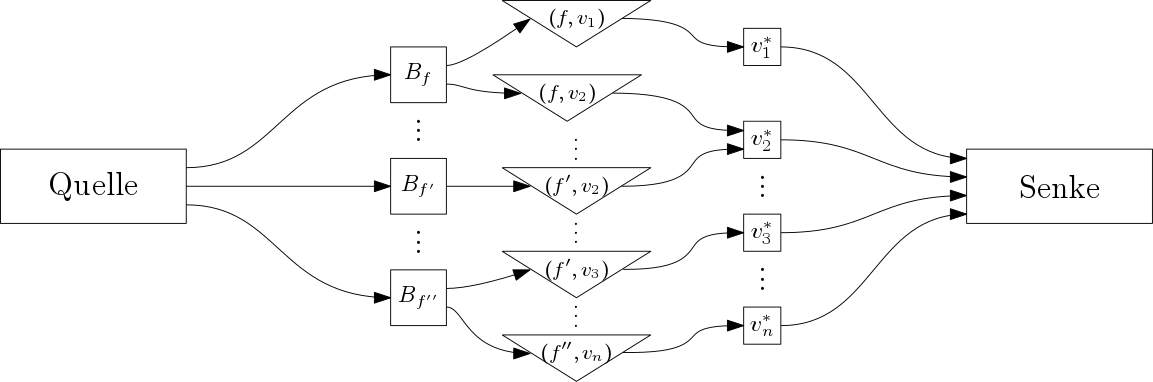
\includegraphics[width=0.7\textwidth]{lem_faa_choice.png}
  	\caption{Skizze des Netzwerkes $\mathcal{F}_z$. Die Kanten von der Quelle zu einem Beutel $B_f$ hat Kapazität $|f|-3$ und alle anderen haben Kapazität 1.}
\end{figure}

$\phi$ weißt nun jedem inneren Gebiet $f$ genau $|f|-3$ Winkel zu und nach Konstruktion kann jeder Knoten $v$ nur einmal zugewiesen werden. Wenn wir noch die per Konstruktion von $\mathcal{N}_G$ zugewiesenen Knoten am äusseren Gebiet hinzunehmen, dann kodiert $\phi$ ein FAA von $G$.
\end{proof}

Wenn wir zeigen können, dass das so erhaltene $\phi$ ein Gutes-FAA ist, folgt Vermutung \ref{int_conj}, da die Existenz eines Guten-FAAs $\phi$ nach Theorem \ref{theo_algo} auch die Existenz eines ganzzahligen zulässigen Flusses $\varphi$ für $\mathcal{N}_G$ impliziert. Ein Weg, zu zeigen 

\begin{lemma}\label{lem_schnyder}
Sei $\tilde{\varphi}$ ein nicht ganzzahliger zulässiger Fluss auf $\mathcal{N}_G$ und sei $C$ die Menge der vom Eckensfluss $\tilde{\varphi}_e$ genutzten inneren Winkel von $G$. Dann existiert eine Teilmenge $\phi\subseteq W$, sodass aus jedem Gebiet $f$ genau $|f|-3$ Winkel in $\phi$ enthalten sind und in der jeder Knoten $v$ höchstens einmal vorkommt. $\phi$ kodiert also ein FAA von $G$.
\end{lemma}

\begin{figure}
\centering
\begin{subfigure}{.4\textwidth}
  \centering
  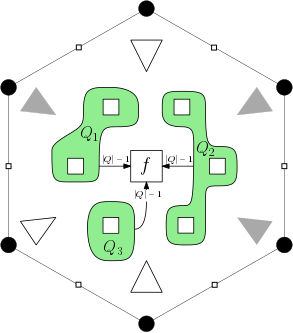
\includegraphics[width=0.9\linewidth]{6_face.png}
\end{subfigure}%
\begin{subfigure}{.6\textwidth}
  \centering
  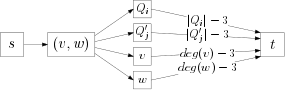
\includegraphics[width=0.9\linewidth]{schnyder_flow_non_int.png}
\end{subfigure}
\caption{Auf der linken Seite eine Illustration von $\overline{\varphi}_s$ mit den von $\overline{\varphi}_z$ zugeordneten Winkeln in grau. Auf der rechten Seite das resultierende Netzwerk.}
\end{figure}

Nehmen wir an wir haben einen Graphen $G$ gefunden für den nur eine nicht ganzzahlige Lösung existiert. Sei $\tilde{\varphi}$ dieser nicht ganzzahlige zulässige Fluss auf $\mathcal{N}_G$, und $\phi$ ein wie in Lemma \ref{lem_faa} aus $\tilde{\varphi}$ konstruiertes FAA für $G$. Sei $\overline{\varphi}_z$ der eindeutige Zuweisungs-Fluss der dieses FAA auf $\mathcal{N}_G$ kodiert. Betrachte nun $\overline{\mathcal{N}}_G$, ein Teilnetzwerk von $\mathcal{N}_G$, aus welchem alle Kanten, die von $\overline{\varphi}_z$ genutzt werden gelöscht wurden. Die Bedarfe sind weiterhin $|E_{in}|$ und $3|F_{in}|$ für den Schnyder- und Ecken-Fluss. Nach der in O1 festgehaltenen Beobachtung können wir, wie in \cite{af15}, $\varphi_s$ und $\varphi_e$ zusammenfassen und mit $\varphi_1$ bezeichnen. Wir suchen also nach einem zulässigem ganzzahligem Fluss $\varphi_1 = \varphi_s + \varphi_e$ auf $\overline{\mathcal{N}}_G$ mit Bedarf $|E_{in}| + 3|F_{in}|$, da dann auch eine ganzzahlige Lösung $(\varphi_s,\varphi_e)$ folgt.

Bevor wir fortfahren wollen wir einige Kantentypen aus $\mathcal{N}_G$ benennen.

\begin{itemize}
\item $E_\triangle = $ Die äusseren Kanten in den Winkeldreiecken.
\item $E_\triangledown = $ Die inneren Kanten in den Winkeldreiecken.
\item $S_* =$ Die Kanten von den Dummy-Knoten zur Dummy-Senke.
\item $V_* = $ Die Kanten von den Winkeldreiecken zu den Dummy-Knoten.
\item $E_{\to} = $ Die Kanten von Quelle 1 zu den Kanten-Knoten.
\item $F_\square = $ Die Kanten von den kleinen Quadraten zu inneren Gebieten $f$.
\item $V_{\to} = $ Die Kanten von den Knoten-Knoten zu Senke 1.
\end{itemize}

Sei $e_{d}$ die Kante von der Dummy-Senke zu Senke 2, dann sind sowohl $\mathcal{S}_1 = E_\triangle \cup E_{\to}$, als auch $\mathcal{S}_2 = F_\square \cup V_{\to} \cup \{e_{d}\}$ minimale Schnitte in $\mathcal{N}_G$, die alle Quellen und Senken trennen. Wenn wir nur von den Kanten aus $E_\triangle$, die in $\overline{\mathcal{N}}_G$ übrig sind, sprechen, schreiben wir $\overline{E}_\triangle$. Für die, zu diesen korrespondierenden Kanten im inneren ihrer Winkeldreiecke, schreiben wir $\overline{E}_\triangledown$. Für die Teilmengen von $V_*$ und $S_*$ in $\overline{\mathcal{N}}_G$ schreiben wir $\overline{S}_*$ und $\overline{V}_*$. Die restlichen Mengen sind vollständig in $\overline{\mathcal{N}}_G$ enthalten.

Seien $E_z$ die von $\overline{\varphi}_z$ genutzen Kanten, die wir aus $\mathcal{N}_G$ entfernen. Dann folgt $|\mathcal{S}_1 \cap E_z| = |E_\triangle \cap E_z| = |\varphi_z|$. Somit ist $\overline{\mathcal{S}}_1 = \mathcal{S}_1 \backslash E_z = \overline{E}_\triangle \cup E_\to$ ein Schnitt in $\overline{\mathcal{N}}_G$. Analog ist $\overline{\mathcal{S}}_2 = F_\square \cup V_{\to}$ ein Schnitt. Für die Kapazität von $\overline{\mathcal{S}}_1$ können wir folgern 
$$ c(\overline{\mathcal{S}}_1) = c(\overline{E}_\triangle) + c(E_\to) = c(E_\triangle) - |\varphi_z| + c(E_\to) = 3|F_{in}| + |E_{in}|,$$
und analog folgt $c(\overline{\mathcal{S}}_2) = 3|F_{in}| + |E_{in}|$.

Falls es sich hierbei um minimale Schnitte handelt, dann würde dies bedeuten, dass eine ganzzahlige Lösung für $\overline{\mathcal{N}}_G$ existiert, mit deren Hilfe wir, zusammen mit $\varphi_z$, eine ganzzahlige zulässige Lösung für $\mathcal{N}_G$ konstruieren könnten, was wiederum ein Widerspruch zu unserer Annahme wäre. Es muss also einen kleineren Schnitt $\mathcal{S}_{min}$, mit $|\mathcal{S}_{min}| \leq 3|F_{in}| + |E_{in}| - 1$, geben. 

\begin{claim} \label{cut_types1}

Ein minimaler Schnitt $\mathcal{S}_{min}$ in $\overline{\mathcal{N}}_G$ enthält ohne Beschränkung der Allgemeinheit nur Kanten von einem der vier Typen $\overline{E}_\triangledown, F_\square, V_\to$ und $E_\to$.

\end{claim}

Kanten auf einem Pfad von der Quelle bis zu einer Kante in $\overline{E}_\triangledown$, können durch diese ersetzt werden. Ebenso können Kanten zwischen zwei Winkeldreiecken, oder von einem Winkeldreieck zu einem kleinen Quadrat, durch die, entgegen dem Uhrzeigersinn, nächste Kante in $\overline{E}_\triangledown$ ersetzt werden. Kanten zwischen einem Kanten-Knoten und einem Knoten-Knoten, oder einem kleinen Quadrat, können durch eine Kante in $E_\to$ ersetzt werden. Abschliessend können Kanten, von einem inneren Gebiet zu Senke, durch das hinzufügen von allen Kanten aus $F_\square$ an diesem Gebiet, ersetzt werden.

\begin{figure}[h]
	\centering
  	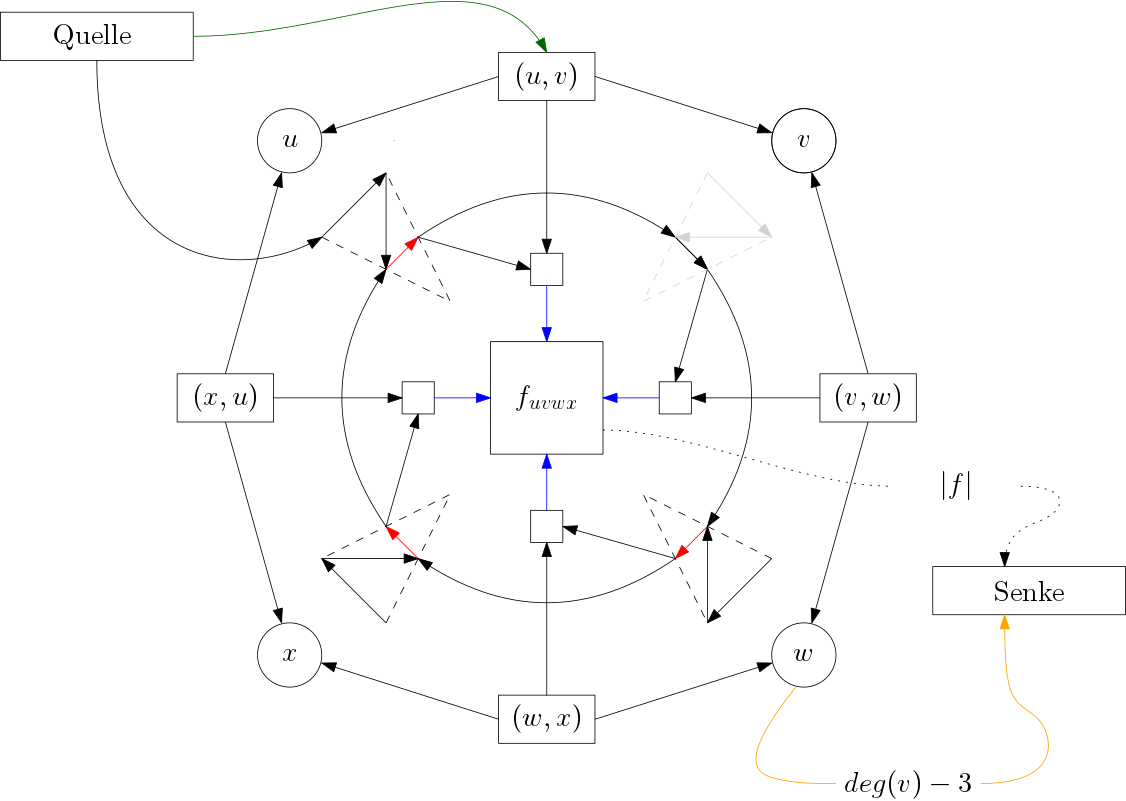
\includegraphics[width=0.7\textwidth]{face_cut.png}
  	\caption{Die vier Kantentypen $\overline{E}_\triangledown$ (rot), $F_\square$ (blau), $V_\to$ (orange) und $E_\to$ (grün) aus denen sich, nach Behauptungen \ref{cut_types1} und \ref{cut_types2}, ein minimaler Schnitt in $\overline{\mathcal{N}}_G$ zusammensetzt.}
\end{figure}

\begin{claim}\label{cut_types2}

Ein minimaler Schnitt $\mathcal{S}_{min}$ in $\overline{\mathcal{N}}_G$ muss ohne Beschränkung der Allgemeinheit aus jeder der Mengen $\overline{E}_\triangledown, F_\square, V_\to$ und $E_\to$ mindestens eine, aber aus keiner der Mengen alle Kanten enthalten.

\end{claim}

Falls ein solcher ein Schnitt existiert, dann kann er nicht alle Kanten $\overline{E}_\triangledown$ enthalten, da sonst $\mathcal{S}_{min} \cup (E_\triangle \cap E_z) \supseteq \mathcal{S}_1$ gilt. Falls er jedoch keine Kante aus $\overline{E}_\triangledown$ enthält, dann muss er alle Kanten aus $F_\square$ enthalten und falls er alle Kanten aus $F_\square$ enthält, dann muss er o.B.d.A. auch alle Kanten aus $V_\to$ enthalten. Es folgt $\mathcal{S}_{min} \cup \{e_d\} \supseteq \mathcal{S}_2$. Angenommen er enthält keine Kante aus $F_\square$, dann muss er alle Kanten aus $\overline{E}_\triangledown$ und $E_\to$ enthalten und es gilt $\mathcal{S}_{min} \cup (E_\triangle \cap E_z) \supseteq \mathcal{S}_1$. Mit analogen Argumenten folgt der Rest von Behauptung \ref{cut_types2}. \\

Nehmen wir also an, dass ein minimaler Schnitt $\mathcal{S}_{min}$, wie in Behauptungen \ref{cut_types1} und \ref{cut_types2}, existiert mit $|\mathcal{S}_{min}| \leq 3|F_{in}| + |E_{in}| - 1$. Betrachten wir für den Moment das Teilnetzwerk um ein inneres Gebiet in $\overline{\mathcal{N}}_G$. Falls alle drei Kanten aus $\overline{E}_\triangledown$ in $\mathcal{S}_{min}$ enthalten sind, dann müssen auch o.B.d.A alle Kanten in $E_\to$ um dieses Gebiet enthalten sein und falls eine Kante aus $\overline{E}_\triangledown$ nicht enthalten ist, dann müssen, im Uhrzeigersinn bis zur nächsten enthaltenen Kante aus $\overline{E}_\triangledown$, alle Kanten aus $F_\square$ Teil von $\mathcal{S}_{min}$ sein. Falls höchstens eine Kante aus $\overline{E}_\triangledown$ im Schnitt läge, dann folgt o.B.d.A, dass keine Kante aus $\overline{E}_\triangledown$ und alle aus $F_\square$, um das innere Gebiet, enthalten sind. 

Angenommen es existieren nur Gebiete in denen entweder alle oder keine Kanten aus $\overline{E}_\triangledown$ in $\mathcal{S}_{min}$ enthalten sind. Dann existiert ein Kanten-Knoten der, wie in Abbildung \ref{face_cut_edge} jeweils eines von beiden berührt. Wir können nun im rechten Gebiet eine Kante aus $F_\square$ durch die, entgegen dem Uhrzeigersinn, folgende Kante aus $\overline{E}_\triangledown$ ersetzen.

Sei $f$ ein Gebiet, 

\begin{figure}[h]
	\centering
  	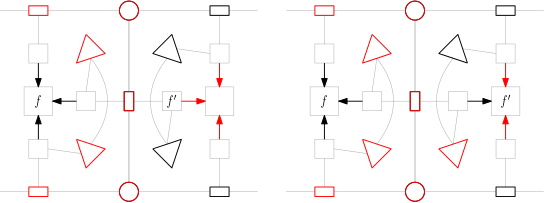
\includegraphics[width=1\textwidth]{sketch_cut.png}
  	\caption{}
	\label{face_cut_edge}
\end{figure}











\begin{lemma}\label{lem_min_cut}
Sei $\mathcal{N}$ ein gerichtetes Netzwerk mit einer Quelle $s$ und einer Senke $t$. Sei $\mathcal{S}_{min}$ ein minimaler Kantenschnitt zwischen $s$ und $t$ und sei $\mathcal{T} \subseteq \mathcal{S}_{min}$. Dann ist $\tilde{\mathcal{S}}_{min} = \mathcal{S}_{min} \backslash \mathcal{T}$ ein minimaler Kantenschnitt zwischen $s$ und $t$ in $\tilde{\mathcal{N}} = \mathcal{N}\backslash \mathcal{T}$.
\end{lemma}

\begin{proof}
Nehmen wir ohne Beschränkung der Allgemeinheit an, dass $\mathcal{N}$ nur Kanten mit Kapazität 1 enthält. Nach dem \textit{Max-Flow Min-Cut} Theorem existiert ein $s$-$t$-Fluss $\varphi$ mit $|\varphi| = c(\mathcal{S}_{min})$. Nach Theorem \ref{theo_int_flow} können wir annehmen, dass wir es sich um einen ganzzahligen Fluss handelt. Wir können diesen Fluss somit in Pfade (TODO) $p$ mit Flussstärke 1 aufteilen. Betrachten wir nun $\tilde{\mathcal{N}} = \mathcal{N} \backslash \mathcal{T}$, dann trennt die Entnahme von $\mathcal{T}$ genau $c(\mathcal{T})$ Pfade $p \in P$. Die restlichen Pfade, nennen wir sie $\tilde{p} \in \tilde{P}$, bleiben intakt. Somit existiert ein $s$-$t$-Fluss $\tilde{\varphi}$ mit $|\tilde{\varphi}| = c(\mathcal{S}_{min}) - c(\mathcal{T})$. $\tilde{\mathcal{S}}_{min} = \mathcal{S}_{min} \backslash \mathcal{T}$ muss somit ein minimaler Schnitt in $\tilde{\mathcal{N}}$ sein, da jedes $p \in \tilde{P}$ genau eine Kante aus $\tilde{\mathcal{S}}_{min}$ nutzt und die Entnahme dieser Kanten, nach Voraussetzung, $s$ und $t$ trennt.
\end{proof}

\begin{lemma}
Sei $\tilde{\varphi}$ ein nicht ganzzahliger zulässiger Fluss auf $\mathcal{N}_G$, dann existiert auch mindestens ein ganzzahliger zulässiger Fluss $\varphi$ auf $\mathcal{N}_G$ und somit auch eine SLTR von $G$.
\end{lemma}

\begin{proof}
Sei $\tilde{\varphi}$ ein nicht ganzzahliger zulässiger Fluss auf $\mathcal{N}_G$ und seien $\overline{P}_*$ und $\overline{V}_*$ die nicht von $\tilde{\varphi}$, also genauer von $\tilde{\varphi}_z$, genutzten Kanten aus $P_*$ und $V_*$. Sei nun $\tilde{\mathcal{N}}_G \subseteq \mathcal{N}_G$ ein Netzwerk, bei dem alle Kanten $e \in \overline{P}_*\cup\overline{V}_*$ aus $\mathcal{N}_G$ gelöscht werden. $\tilde{\varphi}$ ist also weiterhin eine zulässige, nicht ganzzahlige Lösung für $\tilde{\mathcal{N}}_G$.

Betrachten wir für einen Moment das Netzwerk $\tilde{\mathcal{F}}_G$, welches entsteht, wenn wir die Quellen und Senken von $\tilde{\mathcal{N}}_G$ vereinen und nur einen Fluss zwischen der Super-Quelle $s$ und der Super-Senke $t$ betrachten. $\mathcal{S}_1$ und $\mathcal{S}_2$ sind weiterhin minimale Schnitte in $\tilde{\mathcal{F}}_G$ und nach Lemma \ref{lem_min_cut} gilt für jede Teilende $\tilde{\mathcal{S}} \subseteq \mathcal{S}_1$


und $\tilde{\psi} = \tilde{\varphi}_1+ \tilde{\varphi}_2$ ein zulässiger, nicht ganzzahliger Fluss auf $\tilde{\mathcal{F}}_G$. Nach Theorem \ref{theo_int_flow} existiert somit ein zulässiger und ganzzahliger $s$-$t$-Fluss $\psi$ mit $|\psi| = |\tilde{\psi}| = |\tilde{\varphi}|.$ Der Fluss $\psi$ saturiert, da $\mathcal{S}_2$ ein minimaler Schnitt ist, die Kante $e_d$ zwischen der Dummy-Senke und der Senke $t$ und wir können diesen Teil des Flusses $\psi_z$ in $\sum_{f \in F_{in}}(|f|-3)=n$ Pfade $\{p_1, ... ,p_n\} = P$ mit Flussstärke 1 aufteilen. Jeder dieser Pfade $p_i$ führt nun genau durch einen Knoten $v_i^*$ und einen zugehörigen Winkel $(f_i,v_i)$. Es bleibt zu zeigen, dass durch jedes innere Gebiet $f_i$ in $\tilde{\mathcal{F}}_G$ genau $|f_i|-3$ Pfade aus $P$ führen.

Die Menge der genutzten Winkel $\phi$ kodiert nach Lemma \ref{lem_faa} ein FAA von $G$, da es sich um eine Teilmenge der von $\tilde{\varphi}_z$ genutzten Winkel handeln muss. Alle anderen, in $\mathcal{N}_G$ möglichen, Pfade zur Dummy-Senke durch die restlichen Winkel wurden, um $\tilde{\mathcal{F}}_G$ zu erhalten, durch die Entfernung von $\overline{P}_*$ und $\overline{V}_*$ getrennt und stehen für $\psi$ und somit für $\psi_z$ nicht zur Verfügung.

Wir können $\psi$ in $\psi_z$ und $\psi_1$ aufteilen. $\psi_1$ ist, ebenso wie $\psi_z$, ganzzahlig. Da wir, um $\tilde{\mathcal{N}}_G$ zu erhalten, nur Kanten gelöscht haben, welche weder von $\psi_z$, noch von $\psi_1$ genutzt werden, bildet $\varphi_\psi = (\psi_1,\psi_z)$ einen ganzzahligen Zwei-Fluss auf $\tilde{\mathcal{N}}_G$ und somit auch auf $\mathcal{N}_G$. Für diesen Fluss gilt
$$ |\varphi_\psi| = |\psi_1|+|\psi_z| = |\psi| = |\tilde{\varphi}|. $$
Somit handelt es sich bei $\varphi_\psi$ um eine zulässige ganzzahlige Lösung auf $\mathcal{N}_G$ und nach Theorem \ref{theo_algo} existiert somit eine SLTR für $G$.
\end{proof}

Wir haben somit gezeigt, dass mindestens eine Auswahl der Winkel ein Gutes-FAA kodiert. Dies schließt den Beweis von Vermutung \ref{int_conj} fast ab. Der einzige Punkt, der zu zeigen bleibt ist, dass eine beliebige Auswahl der Winkel aus $W$ uns ein Gutes-FAA gibt.

